
% Seções são adicionadas para organizar sua apresentação em blocos discretos, todas as seções e subseções são automaticamente exibidas no índice como uma visão geral da apresentação, mas NÃO são exibidas como slides separados.

\section{Introdução}

%----------------------------------------------------------------------------------------
% \subsection{Contexto}

\begin{frame}{Contexto}
    \begin{itemize}
        \item Na \textbf{computação gráfica}, a representação realista de cenas tridimensionais depende da modelagem da interação entre a luz e os materiais que compõem os objetos.
        \item Profissionais e pesquisadores modelam essa interação por meio das \textbf{funções de distribuição de refletância bidirecional} (BRDFs) \footnote{\tiny{Do inglês, \textit{Bidirectional Reflectance Distribution Functions}. Referência: \cite{pbr}}}.
        \item BRDFs são implementadas em programas especializados que rodam na GPU.
    \end{itemize}
\end{frame}


\begin{frame}{Contexto - BRDF Blinn-Phong}
    \begin{columns}
        % Coluna de texto
        \column{0.5\textwidth}
        \vspace{-0.55cm}
        \hspace{1.65cm}
        \begin{figure}
            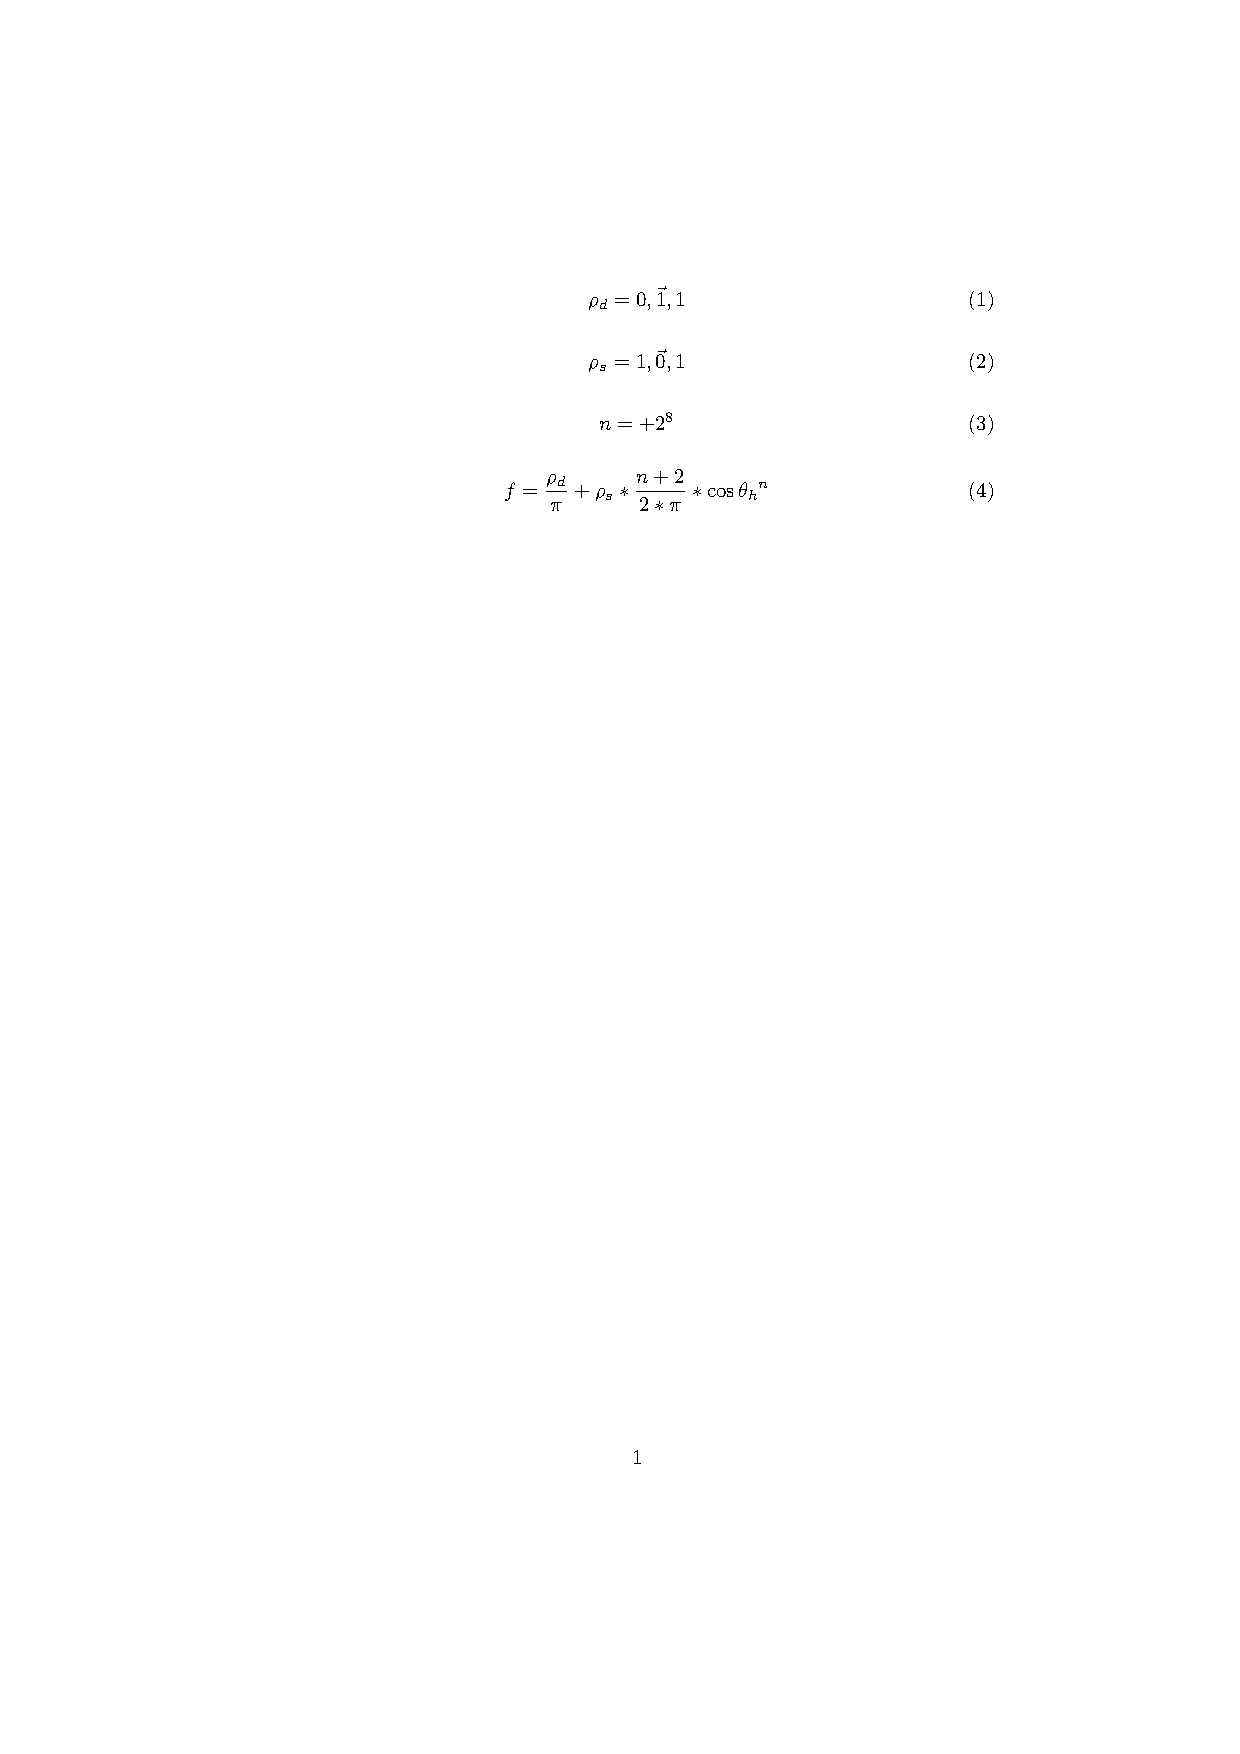
\includegraphics[scale=0.55]{./Imagens/brdfs/blinn-phong.pdf}
        \end{figure}
        
        % Coluna de figuras
        \column{0.5\textwidth}
        \vspace{-0.50cm}
        \begin{figure}[H]
            \centering
            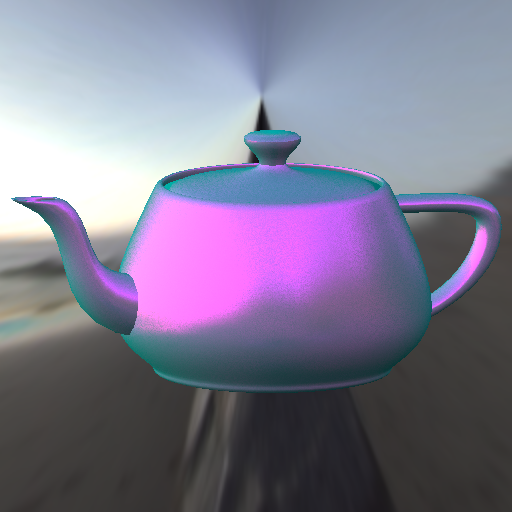
\includegraphics[height=0.32\textheight]{./Imagens/brdfs/blinn-phong-teapot.png}
            
            % {\tiny (a) \textit{Teapot}}
            
            % \vspace{0.1cm}
            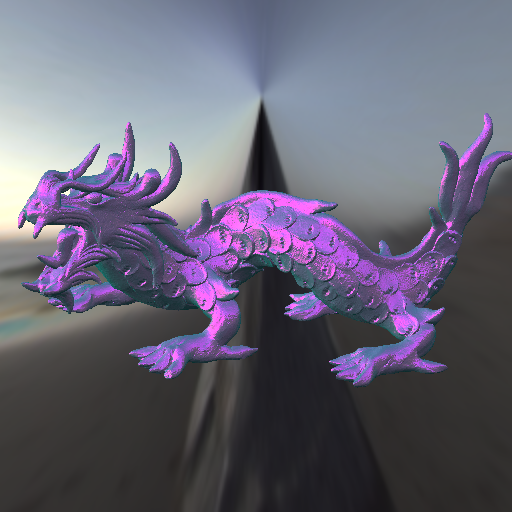
\includegraphics[height=0.32\textheight]{./Imagens/brdfs/blinn-phong-dragon.png}
            
            % \vspace{-0.5cm}
            % {\tiny (b) Dragão de Stanford}
            
            % \vspace{0.1cm}
            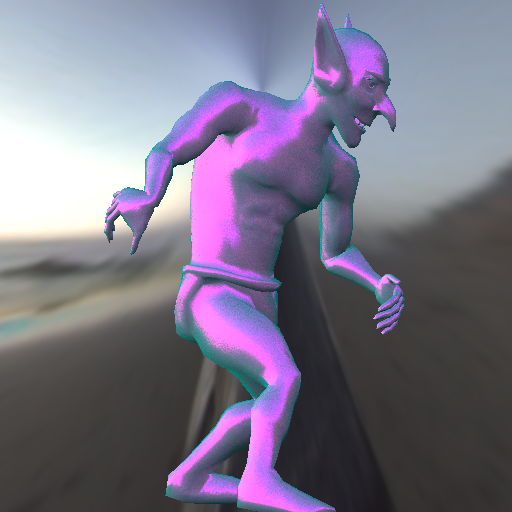
\includegraphics[height=0.32\textheight]{./Imagens/brdfs/blinn-phong-goblin.png}
            
            % \vspace{-0.4cm}
            % {\tiny (c) Goblin}
        \end{figure}
    \end{columns}
\end{frame}

\begin{frame}{Contexto - BRDF Cook-Torrance}
    \begin{columns}
        % Coluna de texto
        \column{0.5\textwidth}
        \small{}
        \vspace{-0.55cm}
        \begin{figure}
            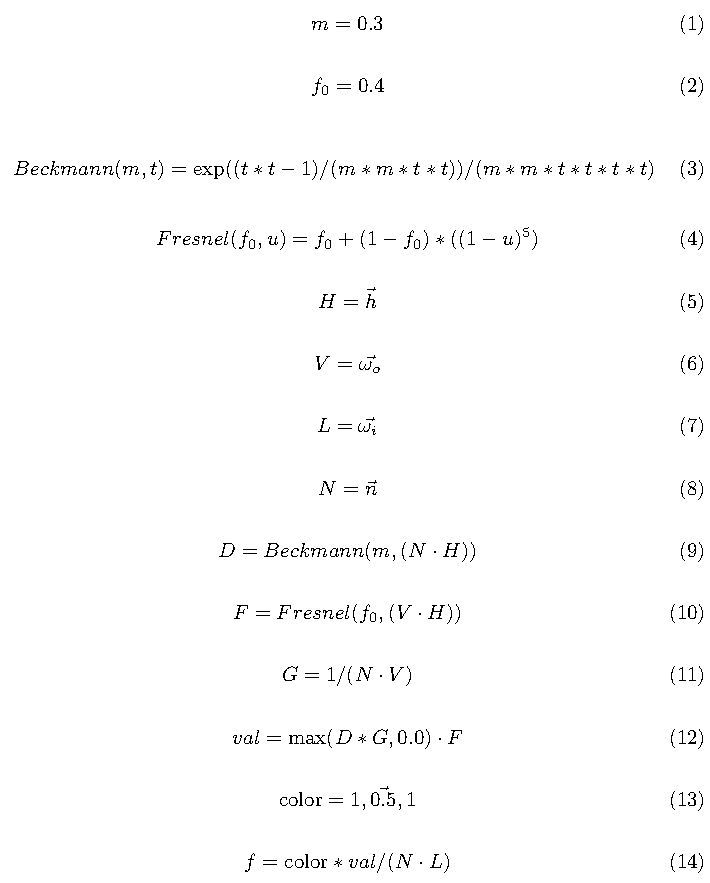
\includegraphics[scale=0.48]{./Imagens/brdfs/cook-torrance-alternative.pdf}
        \end{figure}
        
        % Coluna de figuras
        \column{0.5\textwidth}
        \vspace{-0.50cm}
        \begin{figure}[H]
            \centering
            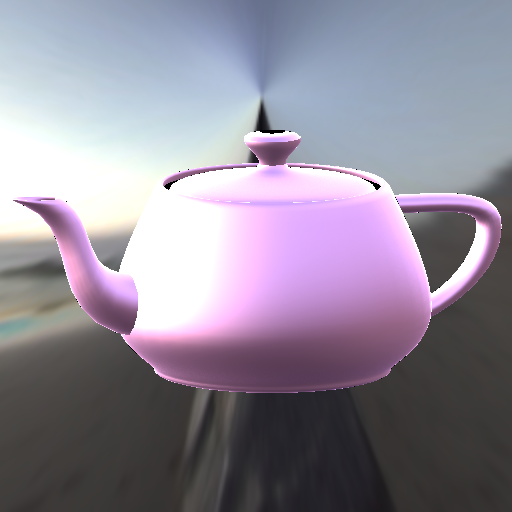
\includegraphics[height=0.32\textheight]{./Imagens/brdfs/cook-torrance-alternative-teapot.png}
            
            % {\tiny (a) \textit{Teapot}}
            
            % \vspace{0.1cm}
            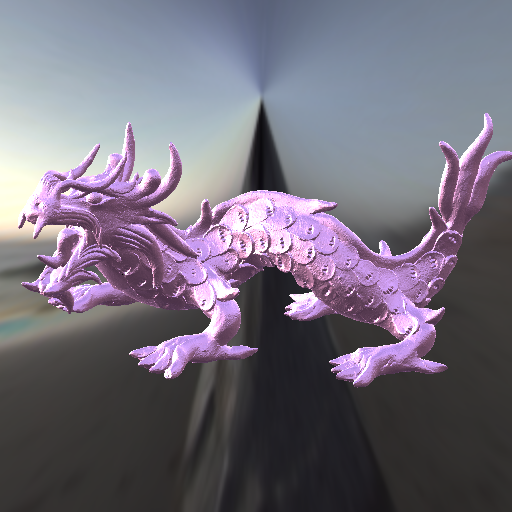
\includegraphics[height=0.32\textheight]{./Imagens/brdfs/cook-torrance-alternative-dragon.png}
            
            % \vspace{-0.5cm}
            % {\tiny (b) Dragão de Stanford}
            
            % \vspace{0.1cm}
            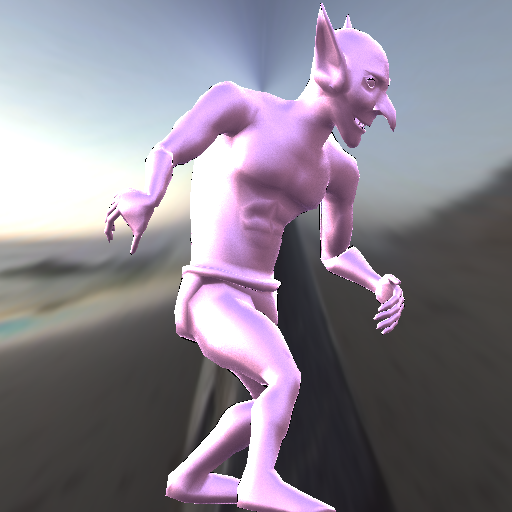
\includegraphics[height=0.32\textheight]{./Imagens/brdfs/cook-torrance-alternative-goblin.png}
            
            % \vspace{-0.4cm}
            % {\tiny (c) Goblin}
        \end{figure}
    \end{columns}
\end{frame}


\begin{frame}{Contexto - \textit{shaders}}
\begin{itemize}
\item \textit{Shaders} concedem a capacidade de cada objeto renderizado ter sua \textbf{aparência configurada por meio de um código} que implementa uma BRDF.
\end{itemize}

\end{frame}

\begin{frame}{Motivação}

    Na renderização, as BRDFs são implementadas por meio de programas chamados de \textit{\textbf{shaders}}. Mas, as BRDFs são comumente descritas por equações em \LaTeX \footnote{\tiny{ \LaTeX{} é um sistema de preparação de documentos para alta qualidade tipográfica. Assim como visto no início.}}. Dois problemas surgem com essa modelagem:

    \begin{enumerate}
        \item Barreira técnica\footnote{\tiny{Físicos ou matemático podem trabalhar com BRDFs e não, necessárimente saber programação baixo nível }}: visualizar essa modelagem de BRDFs requer conhecimento especializado em programação em linguagem de \textit{shading}.
    \item Baixo nível de iteração: toda mudança nas equações exige baixar o nível e reescrever o \textit{shader} novamente.
    \end{enumerate}

\end{frame}


\begin{frame}{Motivação}
        Surge a necessidade de \textbf{simplificar} a \textbf{criação de shaders para BRDFs}. \\\hspace{2cm}


    Um \textbf{compilador} capaz de traduzir BRDFs escritas em \LaTeX{} para \textit{shaders} permitiria uma maior acessibilidade e agilidade na criação de efeitos visuais complexos.
    \begin{figure}[H]
        \begin{center}
            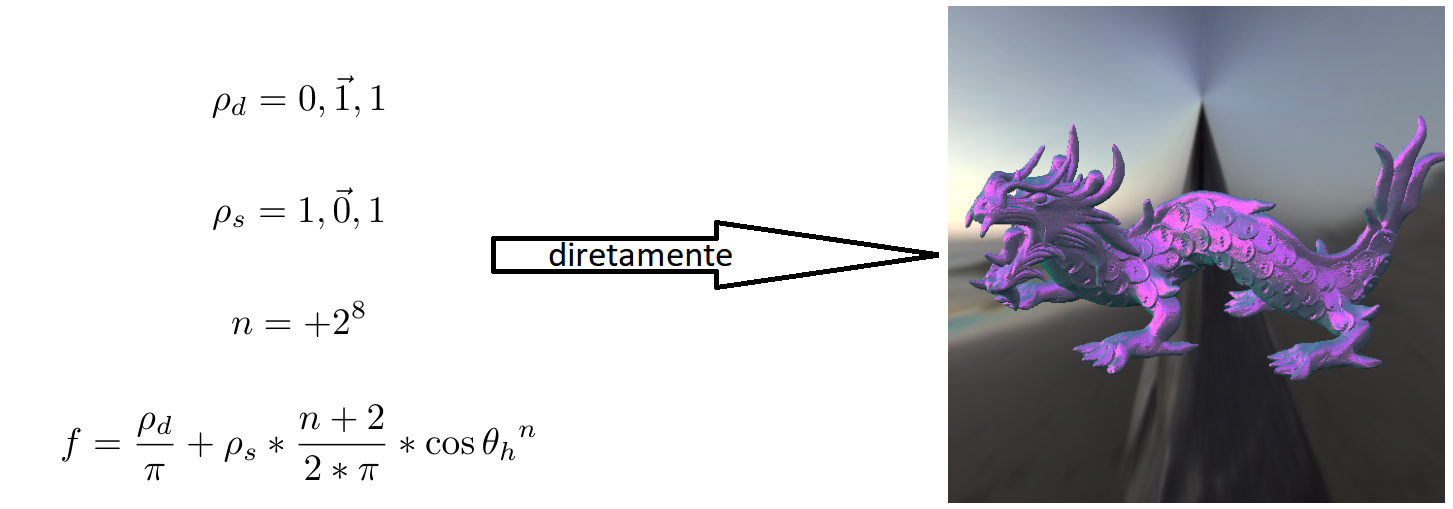
\includegraphics[width=0.65\textwidth]{./Imagens/diretamente.png}
        \end{center}
    \end{figure}
\end{frame}



\begin{frame}{Objetivo}
    Projetar e implementar um \textbf{compilador} capaz de:

    \begin{enumerate}
        \item Processar \textbf{BRDFs} descritas em equações \LaTeX{}.
        \item Gerar \textbf{código de \textit{shading}} na linguagem-alvo da API \textbf{OpenGL}.
        \item Visualizar o efeito dessas BRDFs usando o \textbf{código GLSL} gerado.
    \end{enumerate}

    Resultado esperado é um \textbf{shader} que reproduza as características de refletância da BRDF original.
\end{frame}
